\documentclass[12pt,a4paper,12pt,oneside,openany]{book}
\usepackage{lmodern}
\usepackage{amssymb,amsmath}
\usepackage{ifxetex,ifluatex}
\usepackage{fixltx2e} % provides \textsubscript
\ifnum 0\ifxetex 1\fi\ifluatex 1\fi=0 % if pdftex
  \usepackage[T1]{fontenc}
  \usepackage[utf8]{inputenc}
\else % if luatex or xelatex
  \ifxetex
    \usepackage{mathspec}
  \else
    \usepackage{fontspec}
  \fi
  \defaultfontfeatures{Ligatures=TeX,Scale=MatchLowercase}
    \setmainfont[]{DejaVu Serif}
    \setmonofont[Mapping=tex-ansi,Scale=0.8]{DejaVu Sans Mono}
\fi
% use upquote if available, for straight quotes in verbatim environments
\IfFileExists{upquote.sty}{\usepackage{upquote}}{}
% use microtype if available
\IfFileExists{microtype.sty}{%
\usepackage[]{microtype}
\UseMicrotypeSet[protrusion]{basicmath} % disable protrusion for tt fonts
}{}
\PassOptionsToPackage{hyphens}{url} % url is loaded by hyperref
\usepackage[unicode=true]{hyperref}
\PassOptionsToPackage{usenames,dvipsnames}{color} % color is loaded by hyperref
\hypersetup{
            pdftitle={Devdoc-Swissknife EN},
            pdfauthor={Nikolay Gniteev},
            colorlinks=true,
            linkcolor=Maroon,
            citecolor=Blue,
            urlcolor=Blue,
            breaklinks=true}
\urlstyle{same}  % don't use monospace font for urls
\usepackage{natbib}
\bibliographystyle{apalike}
\usepackage{color}
\usepackage{fancyvrb}
\newcommand{\VerbBar}{|}
\newcommand{\VERB}{\Verb[commandchars=\\\{\}]}
\DefineVerbatimEnvironment{Highlighting}{Verbatim}{commandchars=\\\{\}}
% Add ',fontsize=\small' for more characters per line
\usepackage{framed}
\definecolor{shadecolor}{RGB}{248,248,248}
\newenvironment{Shaded}{\begin{snugshade}}{\end{snugshade}}
\newcommand{\KeywordTok}[1]{\textcolor[rgb]{0.27,0.27,0.27}{\textbf{#1}}}
\newcommand{\DataTypeTok}[1]{\textcolor[rgb]{0.27,0.27,0.27}{#1}}
\newcommand{\DecValTok}[1]{\textcolor[rgb]{0.06,0.06,0.06}{#1}}
\newcommand{\BaseNTok}[1]{\textcolor[rgb]{0.06,0.06,0.06}{#1}}
\newcommand{\FloatTok}[1]{\textcolor[rgb]{0.06,0.06,0.06}{#1}}
\newcommand{\ConstantTok}[1]{\textcolor[rgb]{0,0,0}{#1}}
\newcommand{\CharTok}[1]{\textcolor[rgb]{0.5,0.5,0.5}{#1}}
\newcommand{\SpecialCharTok}[1]{\textcolor[rgb]{0,0,0}{#1}}
\newcommand{\StringTok}[1]{\textcolor[rgb]{0.5,0.5,0.5}{#1}}
\newcommand{\VerbatimStringTok}[1]{\textcolor[rgb]{0.5,0.5,0.5}{#1}}
\newcommand{\SpecialStringTok}[1]{\textcolor[rgb]{0.5,0.5,0.5}{#1}}
\newcommand{\ImportTok}[1]{#1}
\newcommand{\CommentTok}[1]{\textcolor[rgb]{0.37,0.37,0.37}{\textit{#1}}}
\newcommand{\DocumentationTok}[1]{\textcolor[rgb]{0.37,0.37,0.37}{\textbf{\textit{#1}}}}
\newcommand{\AnnotationTok}[1]{\textcolor[rgb]{0.37,0.37,0.37}{\textbf{\textit{#1}}}}
\newcommand{\CommentVarTok}[1]{\textcolor[rgb]{0.37,0.37,0.37}{\textbf{\textit{#1}}}}
\newcommand{\OtherTok}[1]{\textcolor[rgb]{0.37,0.37,0.37}{#1}}
\newcommand{\FunctionTok}[1]{\textcolor[rgb]{0,0,0}{#1}}
\newcommand{\VariableTok}[1]{\textcolor[rgb]{0,0,0}{#1}}
\newcommand{\ControlFlowTok}[1]{\textcolor[rgb]{0.27,0.27,0.27}{\textbf{#1}}}
\newcommand{\OperatorTok}[1]{\textcolor[rgb]{0.43,0.43,0.43}{\textbf{#1}}}
\newcommand{\BuiltInTok}[1]{#1}
\newcommand{\ExtensionTok}[1]{#1}
\newcommand{\PreprocessorTok}[1]{\textcolor[rgb]{0.37,0.37,0.37}{\textit{#1}}}
\newcommand{\AttributeTok}[1]{\textcolor[rgb]{0.61,0.61,0.61}{#1}}
\newcommand{\RegionMarkerTok}[1]{#1}
\newcommand{\InformationTok}[1]{\textcolor[rgb]{0.37,0.37,0.37}{\textbf{\textit{#1}}}}
\newcommand{\WarningTok}[1]{\textcolor[rgb]{0.37,0.37,0.37}{\textbf{\textit{#1}}}}
\newcommand{\AlertTok}[1]{\textcolor[rgb]{0.33,0.33,0.33}{#1}}
\newcommand{\ErrorTok}[1]{\textcolor[rgb]{0.14,0.14,0.14}{\textbf{#1}}}
\newcommand{\NormalTok}[1]{#1}
\usepackage{longtable,booktabs}
% Fix footnotes in tables (requires footnote package)
\IfFileExists{footnote.sty}{\usepackage{footnote}\makesavenoteenv{long table}}{}
\usepackage{graphicx,grffile}
\makeatletter
\def\maxwidth{\ifdim\Gin@nat@width>\linewidth\linewidth\else\Gin@nat@width\fi}
\def\maxheight{\ifdim\Gin@nat@height>\textheight\textheight\else\Gin@nat@height\fi}
\makeatother
% Scale images if necessary, so that they will not overflow the page
% margins by default, and it is still possible to overwrite the defaults
% using explicit options in \includegraphics[width, height, ...]{}
\setkeys{Gin}{width=\maxwidth,height=\maxheight,keepaspectratio}
\IfFileExists{parskip.sty}{%
\usepackage{parskip}
}{% else
\setlength{\parindent}{0pt}
\setlength{\parskip}{6pt plus 2pt minus 1pt}
}
\setlength{\emergencystretch}{3em}  % prevent overfull lines
\providecommand{\tightlist}{%
  \setlength{\itemsep}{0pt}\setlength{\parskip}{0pt}}
\setcounter{secnumdepth}{5}
% Redefines (sub)paragraphs to behave more like sections
\ifx\paragraph\undefined\else
\let\oldparagraph\paragraph
\renewcommand{\paragraph}[1]{\oldparagraph{#1}\mbox{}}
\fi
\ifx\subparagraph\undefined\else
\let\oldsubparagraph\subparagraph
\renewcommand{\subparagraph}[1]{\oldsubparagraph{#1}\mbox{}}
\fi

% set default figure placement to htbp
\makeatletter
\def\fps@figure{htbp}
\makeatother


\title{Devdoc-Swissknife EN}
\author{Nikolay Gniteev}
\date{2021-09-29}

\begin{document}
\maketitle

{
\hypersetup{linkcolor=black}
\setcounter{tocdepth}{2}
\tableofcontents
}
\chapter*{Preface}\label{preface}


This is a demo project for development documentation generation with R Markdown and Kroki

This approach allows you to create reproducible documentation in form of PDF, presentations, gitbook and some other HTML formats from simple markdown-like files (Pandoc flavor) with extra R chunks and textual diagrams description.

The goal of this project is to describe documentation via text files as much as possible, even graphic diagrams, and make it easy to use without overcomplication.

A textual description provides an easy way to version and merge diagrams, get differences between versions, leave comments that stays out from generated documentation, review changes, etc.

Also most often it's faster to create and \textbf{edit} diagrams as text, do things like theming and refactoring themes. Since the diagram's textual description often is more a model than just graphics, you don't have to track existing objects relations when just placement is changed or objects added (until you rename objects) which makes your workflow less error-prone.

R Markdown itself is a powerful and customizable tool, so you can fit docs to your needs. It would take efforts on start, to make things neat but it would repay you in the end.

\begin{quote}
To produce awesome PDFs you'll have to provide awesome Latex book class. Since I don't have one I'm using Latex default so current PDF version looks a bit ugly to me. I hope I can fix this soon or later. Help is appreciated!
\end{quote}

\begin{center}\rule{0.5\linewidth}{\linethickness}\end{center}

This project is also can be used as a template for your own documentation, see \protect\hyperlink{as_template}{this section}

The project uses docker and docker-compose to build docs so it's ready to be integrated into your CI/CD flow.

The project's structure, docs generation and some files are based on \href{https://github.com/rstudio/rmarkdown-book}{R Markdown book}

\begin{center}\rule{0.5\linewidth}{\linethickness}\end{center}

There are few demonstrations in the project for general development use-cases (which probably cover 95\% of your daily needs). For more complicated use-cases - checkout docs on links below.

\begin{quote}
Diagrams code for most examples is borrowed straight from \href{https://kroki.io/examples.html}{Kroki}
\end{quote}

\textbf{Following links would be helpful to you:}

\href{https://kroki.io/\#support}{List of supported diagrams renderers - https://kroki.io/\#support}

\href{https://kroki.io/examples.html}{A few more diagrams examples - https://kroki.io/examples.html}

\href{https://bookdown.org/yihui/rmarkdown/}{R Markdown: The Definitive Guide - https://bookdown.org/yihui/rmarkdown/}\\
created by one of R Markdown authors and generated with R Markdown

\href{https://bookdown.org/yihui/rmarkdown-cookbook/}{R Markdown: Cookbook - https://bookdown.org/yihui/rmarkdown-cookbook/}

\href{https://rmd4sci.njtierney.com/}{A nice R Markdown tutorial - https://rmd4sci.njtierney.com/}

\href{https://raw.githubusercontent.com/rstudio/cheatsheets/master/rmarkdown.pdf}{R Markdown cheatsheet - https://raw.githubusercontent.com/rstudio/cheatsheets/master/rmarkdown.pdf}

\href{https://rmarkdown.rstudio.com/docs/reference/index.html}{R Markdown reference - https://rmarkdown.rstudio.com/docs/reference/index.html}

\href{https://github.com/DaveJarvis/keenwrite}{Keenwrite - edit and preview R Markdown Live!}

\chapter{Simple diagrams examples}\label{simple-diagrams-examples}

Since this project is focused on embedding diagrams text descriptions into R Markdown let's start with few examples just to illustrate a principle.

\section{Example with inline diagram description}\label{example-with-inline-diagram-description}

This example shows how to embed diagrams, describing them right in Rmd file

This code:

\begin{Shaded}
\begin{Highlighting}[]
\StringTok{```}\DataTypeTok{\{r echo=FALSE, results='asis'\}}
\DataTypeTok{  to_diagram("graphviz", "Hello World",}
\DataTypeTok{  "digraph G \{Hello->World\}"}
\DataTypeTok{  )}
\StringTok{```}
\end{Highlighting}
\end{Shaded}

would produce following diagram:

\begin{figure}
\centering
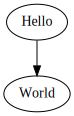
\includegraphics{generated/Hello World.pdf}
\caption{Hello World}
\end{figure}

\begin{quote}
\emph{Take a NOTE: When diagrams are inserted like this it's \textbf{IMPORTANT} that (``Hello World'' in this example) is \textbf{UNIQUE} for \textbf{WHOLE} doc.}\\
More details on usage is in \href{TODO:}{\ldots{}}
\end{quote}

\newpage

\section{Example with diagram data from file}\label{example-with-diagram-data-from-file}

This example shows how to embed diagrams with data from outer files.

This code:

\begin{Shaded}
\begin{Highlighting}[]
\StringTok{```}\DataTypeTok{\{r echo=FALSE, results='asis'\}}
\DataTypeTok{  to_diagram("erd", "Entity Relation", src="../diagrams/examples/project.erd")}
\StringTok{```}
\end{Highlighting}
\end{Shaded}

would produce following diagram:

\begin{figure}
\centering
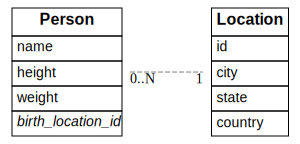
\includegraphics{generated/diagrams-examples-project-erd.pdf}
\caption{Entity Relation}
\end{figure}

\begin{center}\rule{0.5\linewidth}{\linethickness}\end{center}

File \textbf{diagrams/examples/project.erd} content:

\begin{verbatim}
[Person]
*name
height
weight
+birth_location_id

[Location]
*id
city
state
country

Person *--1 Location
\end{verbatim}

\section{More examples}\label{more-examples}

More examples can be found in \protect\hyperlink{examplesKroki}{this section}.

\hypertarget{as_template}{\chapter{Using as a template and making own docs}\label{as_template}}

To use this project as a start point for generating your own documentation do the following:

\begin{enumerate}
\def\labelenumi{\arabic{enumi}.}
\tightlist
\item
  Import project and prepare for making docs
\end{enumerate}

\begin{quote}
You'll need to have already \texttt{docker} and \texttt{docker-compose} installed
\end{quote}

\begin{itemize}
\item
  Import or fork master branch of this repo: \url{https://github.com/Godhart/devdoc-swissknife}\\
  All the sources for docs are contained in \texttt{docs\_src} folder.
\item
  Make a new folder in \texttt{docs\_src}. I suggest you name it using the following pattern: \texttt{doc-\textless{}subject\textgreater{}}
\item
  Copy all the files from \texttt{docs\_src/docs-template} into your brand new folder
\item
  Replace following keywords \texttt{\textless{}Author\ Name\textgreater{}}, \texttt{\textless{}author\textgreater{}}, \texttt{\textless{}repo\textgreater{}}, \texttt{\textless{}Document\ Title\textgreater{}}, \texttt{Document\_Title}, \texttt{\textless{}Document\ Description\textgreater{}}, doc- within files in your new folder with actual values. Don't forget also to adjust \texttt{Document\_Title} in the \texttt{.gitignore} of new folder, as it protects from build garbage.
\item
  If you don't want to see devdoc-swissknife documentation in your repo:

  \begin{itemize}
  \tightlist
  \item
    Remove \texttt{docs\_src/devdoc-swissknife-*} folders
  \item
    Empty \texttt{docs\_src/diagrams} folder.
  \end{itemize}
\item
  Adjust \texttt{docs\_src/Makefile} to fit your needs (for the first time - use an existing pattern to add your folder).
\item
  Make docker image \texttt{devdoc-swissknife} if you don't have one already. Simply run \texttt{make\_docker.sh} from \texttt{docker} dir.
\item
  Try to make docs with \texttt{make\_docs.sh}. Output docs should appear in \texttt{docs\_out/doc-\textless{}subject\textgreater{}} folder if you followed a pattern in the Makefile.\\
  \emph{Take a NOTE: \texttt{docs\_out} folder and all it's content is ignored by git.}
\end{itemize}

\begin{quote}
NOTE: in many cases of errors doc's sources folder is polluted with temporary files, named as specified in \texttt{\_bookdown.yml} (field \texttt{book\_filename}) and may break following docs generation runs.\\
These files are removed with make routine, but in some cases, you'll have to remove them by yourself.\\
Changing \texttt{book\_filename} field in \texttt{\_bookdown.yml} after an error has happened may be the case.
\end{quote}

\begin{enumerate}
\def\labelenumi{\arabic{enumi}.}
\setcounter{enumi}{1}
\tightlist
\item
  Create content
\end{enumerate}

\begin{itemize}
\item
  Update \texttt{index.Rmd} in your folder to your needs (contains \emph{Preface} section).
\item
  Add your own docs into your folder, naming files like \texttt{\textless{}number\textgreater{}-\textless{}chapter-name\textgreater{}.Rmd}.\\
  Check the R Markdown and Kroki docs for understanding things. Also, you may rely on shown examples.
\end{itemize}

*If you already have docs in markdown format you may already use them like this:

\begin{verbatim}
* copy markdown files into your doc-folder
* copy necessary local images to location in `docs_src/diagrams` or wherever you like most
* change name extensions of markdown files to `.Rmd`
* change names of markdown files so they would correspond to pattern `<number>-<chapter-name>.Rmd`
* change references to local images in markdown files
\end{verbatim}

\begin{itemize}
\tightlist
\item
  Most probably you would like to use your own Latex class, so add \texttt{\textless{}your\_latex\_class\textgreater{}.cls} file into your folder and specify it in \texttt{index.Rmd} file (replace \texttt{documentclass:\ book} field with \texttt{\textless{}your\_latex\_class\textgreater{}} name).
\end{itemize}

\begin{quote}
Adding custom latex class may require you to add some latex packages to Docker image. Same is true if you do use some special R packages in your docs etc.\\
If this is the case you'll have to modify \texttt{docker/Dockerfile} and build again docker image with \texttt{make\_docker.sh}.
\end{quote}

\hypertarget{examplesKroki}{\chapter{Kroki usage examples}\label{examplesKroki}}

I've omitted some examples from \href{https://kroki.io/examples.html}{Kroki} and left only those that most useful in a daily life of most developers (IMHO).

If you check docs for \href{https://kroki.io/\#support}{supported diagrams renderers} then you'll find for sure a few more interesting usecases.

All diagrams data for examples of this section resides in \href{https://github.com/Godhart/devdoc-swissknife/tree/main/docs_src/diagrams/examples}{\texttt{docs\_src/diagrams}} dir of this repo. Each diagram is included into doc by adding following code section into document file:

\begin{Shaded}
\begin{Highlighting}[]
\StringTok{```}\DataTypeTok{\{r echo=FALSE, results='asis'\}}
\DataTypeTok{  to_diagram("from_src", "<Drawing name>", src="../diagrams/<src_file_path_within_diagrams_dir>")}
\StringTok{```}
\end{Highlighting}
\end{Shaded}

Full code for this whole section is \href{https://github.com/Godhart/devdoc-swissknife/blob/main/docs_src/devdoc-swissknife-en/03-KrokiExamples.Rmd}{here}

This usage pattern is described in the following section \protect\hyperlink{TODO}{TODO}

\newpage

\section{C4 Context Diagram (PlantUML+C4)}\label{c4-context-diagram-plantumlc4}

Engine: \texttt{c4plantuml}

\begin{figure}
\centering
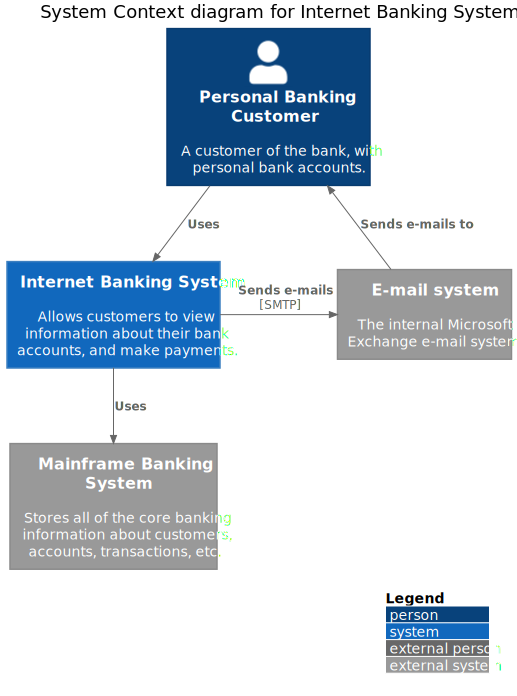
\includegraphics[height=15.00000cm]{generated/diagrams-examples-c4plantuml-context-Rmd.png}
\caption{Example - C4 Context Diagram}
\end{figure}

\begin{quote}
*NOTE: inserted as PNG image due to errors in SVG to PDF conversion
\end{quote}

\newpage

\section{C4 Container Diagram (PlantUML+C4)}\label{c4-container-diagram-plantumlc4}

Engine: \texttt{c4plantuml}

\begin{figure}
\centering
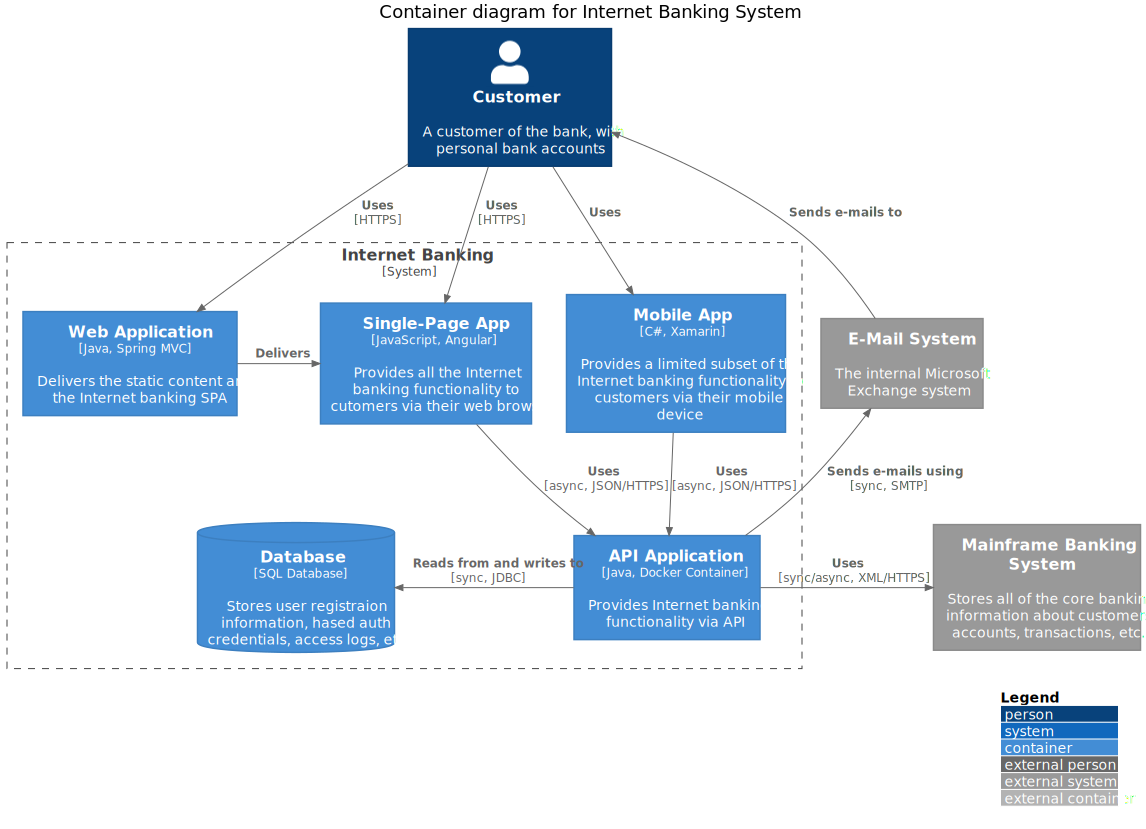
\includegraphics[width=1.00000\textwidth]{generated/diagrams-examples-c4plantuml-container-Rmd.png}
\caption{Example - C4 Container Diagram}
\end{figure}

\begin{quote}
*NOTE: inserted as PNG image due to errors in SVG to PDF conversion
\end{quote}

\newpage

\section{C4 Component Diagram (PlantUML+C4)}\label{c4-component-diagram-plantumlc4}

Engine: \texttt{c4plantuml}

\begin{figure}
\centering
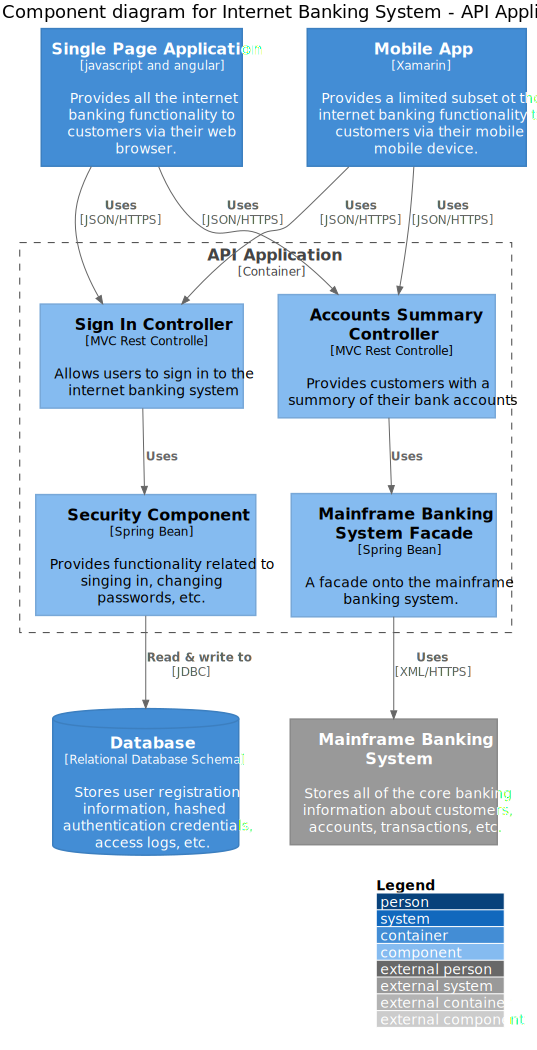
\includegraphics[height=15.00000cm]{generated/diagrams-examples-c4plantuml-component-Rmd.png}
\caption{Example - C4 Component Diagram}
\end{figure}

\begin{quote}
*NOTE: inserted as PNG image due to errors in SVG to PDF conversion
\end{quote}

\newpage

\section{Block Diagram}\label{block-diagram}

Engine: \texttt{blockdiag}

\begin{figure}
\centering
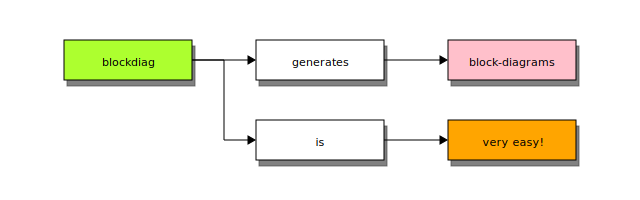
\includegraphics{generated/diagrams-examples-blockdiag-Rmd.pdf}
\caption{Example - Block Diagram}
\end{figure}

\newpage

\section{Digital Timing Diagram}\label{digital-timing-diagram}

Engine: \texttt{wavedrom}

\begin{figure}
\centering
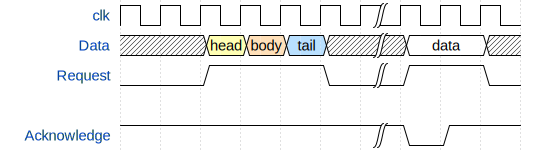
\includegraphics{generated/diagrams-examples-wavedrom-Rmd.pdf}
\caption{Example - Digital Timing Diagram}
\end{figure}

\newpage

\section{Bytefield}\label{bytefield}

Engine: \texttt{bytefield}

\begin{figure}
\centering
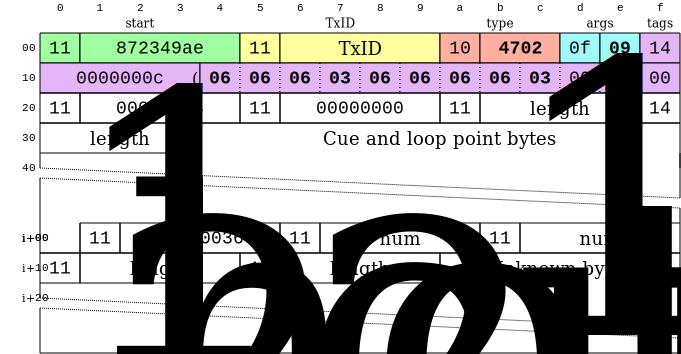
\includegraphics{generated/diagrams-examples-bytefield-Rmd.pdf}
\caption{Example - Bytefield}
\end{figure}

\newpage

\section{Packet Diagram}\label{packet-diagram}

Engine: \texttt{packetdiag}

\begin{figure}
\centering
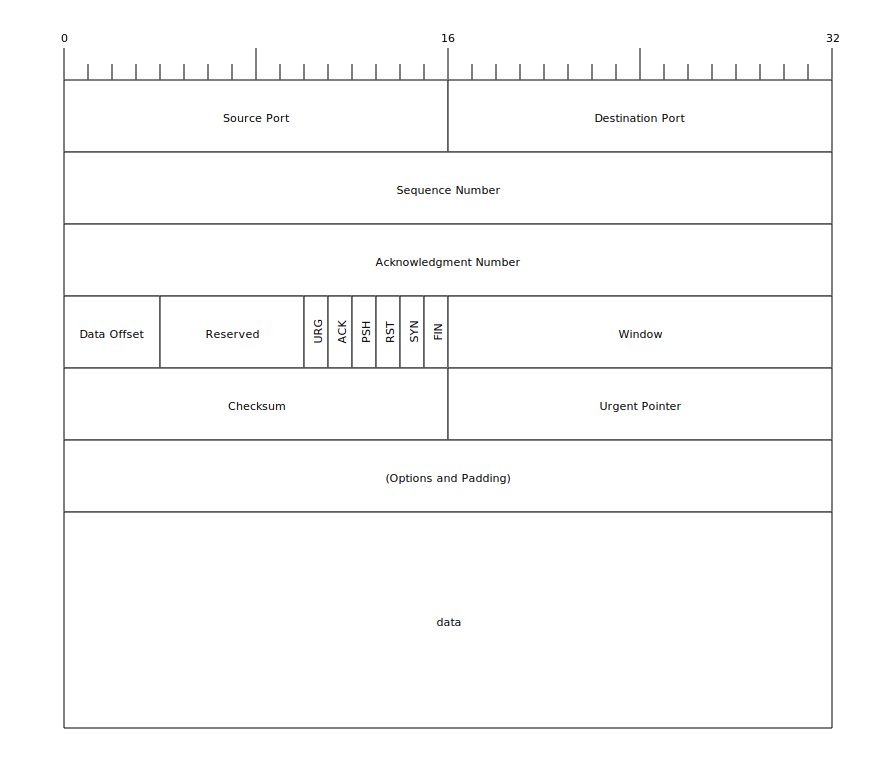
\includegraphics[width=1.00000\textwidth]{generated/diagrams-examples-packetdiag-Rmd.pdf}
\caption{Example - Packet Diagram}
\end{figure}

\newpage

\section{Sequence Diagram \#1 (PlantUML)}\label{sequence-diagram-1-plantuml}

Engine: \texttt{plantuml}

\begin{figure}
\centering
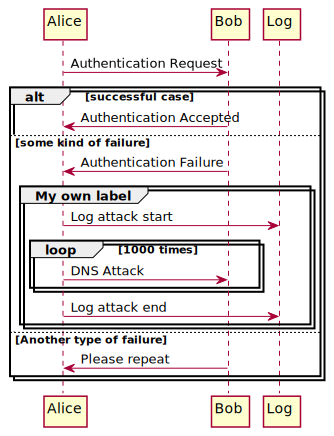
\includegraphics{generated/diagrams-examples-plantuml-seqdiag-Rmd.pdf}
\caption{Example - Sequence Diagram - PlantUML}
\end{figure}

\newpage

\section{Sequence Diagram \#2 (SeqDiag)}\label{sequence-diagram-2-seqdiag}

Engine: \texttt{seqdiag}

\begin{figure}
\centering
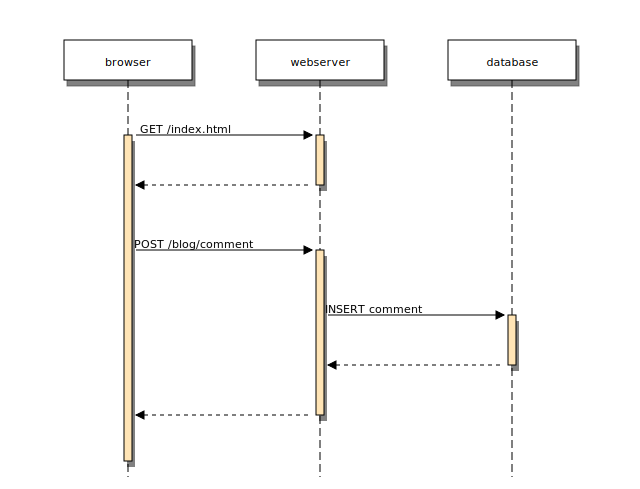
\includegraphics{generated/diagrams-examples-seqdiag-Rmd.pdf}
\caption{Example - Sequence Diagram - SeqDiag}
\end{figure}

\newpage

\section{Commit Graph}\label{commit-graph}

Engine: \texttt{pikchr}

\begin{quote}
\emph{NOTE: pikchr is giving troubles in PDF/PNG (produced SVG output is only web-browser friendly)}
\end{quote}

\newpage

\section{Use Case Diagram}\label{use-case-diagram}

Engine: \texttt{plantuml}

\begin{figure}
\centering
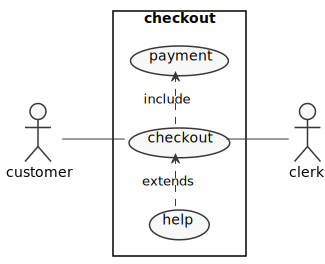
\includegraphics{generated/diagrams-examples-plantuml-usecase-Rmd.pdf}
\caption{Example Block Diagram}
\end{figure}

\newpage

\section{Mind Map}\label{mind-map}

Engine: \texttt{plantuml}

\begin{figure}
\centering
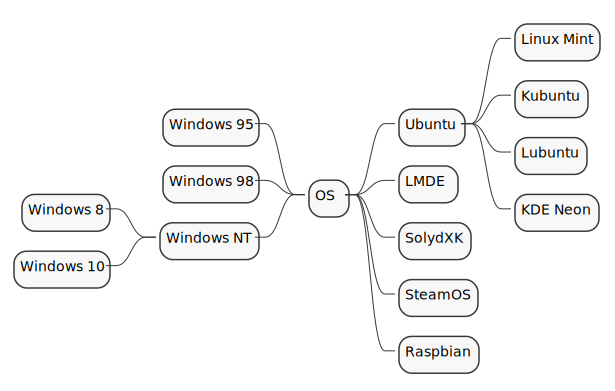
\includegraphics{generated/diagrams-examples-plantuml-mindmap-Rmd.pdf}
\caption{Example - Mind Map}
\end{figure}

\newpage

\section{PlantUML (More examples)}\label{plantuml-more-examples}

PlantUML supports more diagram types like timing diagram, gantt and many more.

You can use any of them just like in previous examples.

Check PlantUML docs \url{https://plantuml.com/} for filling in diagram data.

\newpage

\section{Gantt}\label{gantt}

Engine: \texttt{mermaid}

\begin{quote}
\emph{NOTE: mermaid is giving troubles in PDF/PNG (produced SVG output is only web-browser friendly)}
\end{quote}

\begin{figure}
\centering
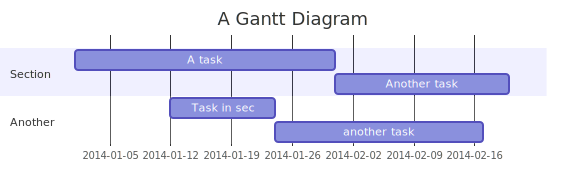
\includegraphics{generated/diagrams-examples-mermaid-gantt-Rmd.pdf}
\caption{Example - Gantt}
\end{figure}

\bibliography{book.bib,packages.bib}

\end{document}
